\documentclass{beamer}
\usefonttheme{professionalfonts}
\usetheme[subsectionpage=progressbar]{metropolis}
\setbeamertemplate{section in toc}[sections numbered]
\setbeamertemplate{subsection in toc}[subsections numbered]

\title{Riemannian Trust-Region SR1 Method}
\subtitle{in \lstinline!Manopt.jl!}
\author{Tom-Christian Riemer}
\institute{TU Chemnitz}
\date{Research Seminar Numeric,\\ 16th June 2021}

%packages
\usepackage{amsmath}
\usepackage[british]{babel}
\usepackage[utf8]{inputenc}
\usepackage{enumerate}
\usepackage{graphicx}
\usepackage{mathtools}
\usepackage{color}
\usepackage{listings}
\usepackage[]{algorithm2e}
\usepackage{numapde-manifolds}

\definecolor{presentationblue}{RGB}{0,119,187}

\lstset{basicstyle=\ttfamily,	tabsize=2}

\newcommand\myeq{\stackrel{\mathclap{\mbox{$def$}}}{=}}

\newcommand{\Pb}[1]{\expandafter\hat#1}

\begin{document}

\maketitle

\begin{frame}{Contents}
	\tableofcontents
\end{frame}

\section{Introduction}

\begin{frame}{Riemannian Optimization}
    Finding a \textbf{minimum} of a real-valued function $f$ on a Riemannian manifold, i.e. \\
    \begin{equation*}
        \min f(x), \quad x \in \mathcal{M}.
    \end{equation*}\\[1.\baselineskip]
    \begin{center}
        \textbf{Riemannian manifold} = smooth manifold + Riemannian metric. \\[1.\baselineskip]
    \end{center}
    \begin{equation*}
        \mathbb{S}^{n-1} = \{ x \in \mathbb{R}^n \colon \; \lVert x \rVert_2 = 1 \}.
    \end{equation*}
\end{frame}

\begin{frame}{Euclidean Trust-Region Methods}
    \alert{Quadratic model} at current iterate:
	\begin{equation*}
    	m_k(s) = f(x_k) + \alert{\nabla f(x_k)}^{\mathrm{T}} s + \frac{1}{2} s^{\mathrm{T}} H_k s.
    \end{equation*}
	Finding a \alert{step} (e.g. with tCG):
	\begin{equation*}
        s_k = \arg \min_{\alert{\lVert} s \alert{\rVert_2} \leq \Delta_k} m_k(s),
    \end{equation*}
	where $\Delta_k > 0$ defines the \alert{trust-region}. \\
    The candidate of the next iterate is
	\begin{equation*}
        \widetilde{x}_{k+1} = \alert{x_k + s_k}.
    \end{equation*}
	We take $\widetilde{x}_{k+1}$ as the next iterate if $\frac{f(x_k) - f(\widetilde{x}_{k+1})}{m_k(0) - m_k(s_k)} =\rho_k > \rho^{\prime}$. \\[0.1\baselineskip]
    Update $\Delta_k \rightarrow \Delta_{k+1}$ depending on $\rho_k$ and $\lVert s_k \rVert_2$.
\end{frame}

\section{RTR-SR1 Method}

\begin{frame}{Tangent Spaces}
    \vspace{-0.5\baselineskip}\hfill{\tiny{[Absil, Mahony, Sepulchre, 2008]}}
    \begin{center}
        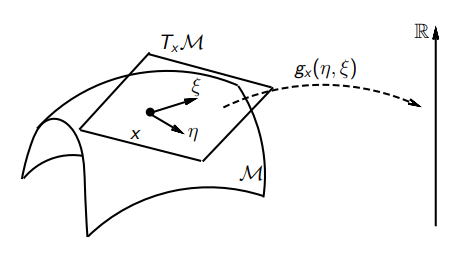
\includegraphics[width=5cm]{img/Riemannian_Metric.png}
    \end{center}
    \textbf{Tangent space} $\tangent{x}$ at $x$ is the set of all tangent vectors (directions) at $x$. $\tangent{x}$ is a linear space. \\[0.2\baselineskip]
    \textbf{Riemannian metric} $g_{\cdot} (\cdot, \cdot)$ is a smoothly-varying inner product on the tangent spaces. Norm: $\lVert \xi_x \rVert_x = \sqrt{g_x(\xi_x, \xi_x)}$. \\[0.2\baselineskip]
    \textbf{Riemannian gradient} $\mathrm{D} \, f(x) [\eta_x] = g_x (\operatorname{grad} f(x), \eta_x),$ \\
    for all $\eta_x \in \tangent{x}$.
\end{frame}

\begin{frame}{Retractions}
    \vspace{-0.5\baselineskip}\hfill{\tiny{[Absil, Mahony, Sepulchre, 2008]}}
    \begin{center}
        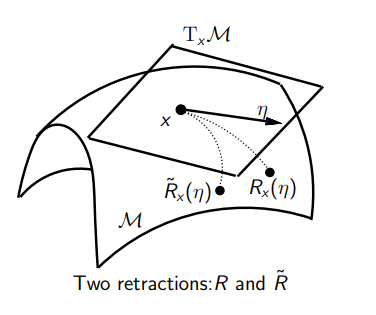
\includegraphics[width=4cm]{img/Retraction.png}
    \end{center}
    A \textbf{Retraction} is a smooth map $R_x \colon \tangent{x} \to \mathcal{M}$, which satisfies \\[-0.1\baselineskip]
    \begin{itemize}
        \item $R_x (0_x) = x$ and
        \item $\mathrm{D} \, R_x (0_x)[\xi_x] = \xi_x,$ for all $\xi_x \in \tangent{x}$.
    \end{itemize}
    \textbf{Pullback} $\widehat{f}_x = f \circ R_x \colon \tangent{x} \to \mathbb{R}$, \\
    $\operatorname{grad} \widehat{f}_x (0_x) = \operatorname{grad} f(x)$ for all $x \in \mathcal{M}$.
\end{frame}

\begin{frame}{Riemannian Trust-Region Methods}
    \vspace{-1.5\baselineskip}
    \begin{align*}
        m_k( s ) & = \widehat{f}_{x_k}(0_{x_k}) + g_{x_k}(\operatorname{grad} \widehat{f}_{x_k}(0_{x_k}), s ) + \frac{1}{2} g_{x_k}( s , \alert{\mathcal{H}_k [} s \alert{]} ) \\
        & = f(x_k) + g_{x_k}(\operatorname{grad} f(x_k), s ) + \frac{1}{2} g_{x_k}( s , \alert{\mathcal{H}_k [} s \alert{]} ) \\
        & \text{Step: } \tangent{x_k} \ni s_k = \arg \min_{\lVert s \rVert_{x_k} \leq \Delta_k} m_k( s ) \\
        & \text{Candidate: } \widetilde{x}_{k+1} = R_{x_k}(s_k)
    \end{align*}
    \textbf{TR Newton Method}: \\
    $\mathcal{H}_k = \operatorname{Hess} f(x_k) \colon \tangent{x_k} \ni \xi_{x_k} \mapsto \nabla_{\xi_{x_k}} \operatorname{grad} f(x_k) \in \tangent{x_k}$. \\[0.2\baselineskip]
	\textbf{TR SR1 Method}: \\
    $\mathcal{H}_k = \mathcal{H}^{SR1}_k \approx \operatorname{Hess} f(x_k)$. \\
    $\mathcal{H}^{SR1}_k \rightarrow \mathcal{H}^{SR1}_{k+1} \colon \alert{\tangent{x_{k+1}}} \to \alert{\tangent{x_{k+1}}}$ \\
    using $s_k, \operatorname{grad} f(x_k) \in \alert{\tangent{x_k}}$ and $\operatorname{grad}f(\widetilde{x}_{k+1}) \in \alert{\tangent{\widetilde{x}_{k+1}}}$.
\end{frame}

\begin{frame}{Vector Transports}
    \vspace{-1\baselineskip}\hfill{\tiny{[Absil, Mahony, Sepulchre, 2008]}}
    \begin{center}
        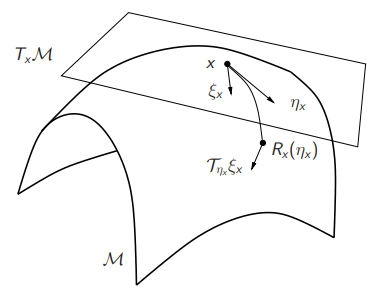
\includegraphics[width=5cm]{img/Vector_Transport.png}
    \end{center}
    \textbf{Vector Transport} is a smooth linear map $T_x \colon \tangent{x} \times \tangent{x} \ni (\eta_x, \xi_x) \mapsto T_{x, \eta_x}(\xi_x) \in \tangent{R_x(\eta_x)}$. \\[0.5\baselineskip]
    \textbf{Isometric VT} satisfies $\lVert \xi_x \rVert_x = \lVert T^{S}_{x, \eta_x}(\xi_x) \rVert_{R_x(\eta_x)}$.
\end{frame}

% The link to the Euclidean variant must still be found, in which it is made clear that eta_k generalizes the distance between x_k and x_k+1. Maybe another slide.
\begin{frame}{Symmetric Rank One Update}
    Let $\nu \in (0,1)$ (e.g. $\nu = 10^{-8}$), $\mathcal{H}^{SR1}_0 [\cdot] = id[\cdot]$. We have
    \begin{align*}
        & s_k \in \tangent{x_k} \quad (\widetilde{x}_{k+1} = R_{x_k}(s_k) \text{ generalizes } \widetilde{x}_{k+1} = x_k + s_k) \\
        & y_k = \alert{{T^{S}_{x_k, s_k}}^{-1} (} \operatorname{grad}f(\widetilde{x}_{k+1}) \alert{)} - \operatorname{grad}f(x_k) \in \tangent{x_k}.
    \end{align*}
    If
    \begin{equation*}
        \lvert g_{x_k}(s_k, y_k - \mathcal{H}^{SR1}_k[s_k]) \rvert \geq \nu \; \lVert s_k \rVert_{x_k} \lVert y_k - \mathcal{H}^{SR1}_k[s_k] \rVert_{x_k},
    \end{equation*}
    then
    \begin{equation*}
        \widetilde{\mathcal{H}}^{SR1}_{k+1} [\cdot] = \mathcal{H}^{SR1}_k [\cdot] + \frac{(y_k - \mathcal{H}^{SR1}_k [s_k]) (y_k - \mathcal{H}^{SR1}_k [s_k])^{\flat} [\cdot] }{(y_k - \mathcal{H}^{SR1}_k [s_k])^{\flat} [s_k]},
    \end{equation*}
    % where $\xi^{\flat}_{x_k} \colon \tangent{x_k} \ni \zeta_{x_k} \mapsto g_{x_k}(\xi_{x_k}, \zeta_{x_k}),$ for all $\xi_{x_k} \in \tangent{x_k}$. \\
    Else 
    \begin{equation*}
        \widetilde{\mathcal{H}}^{SR1}_{k+1} [\cdot] = \mathcal{H}^{SR1}_k [\cdot].
    \end{equation*}
    % $\widetilde{\mathcal{H}}^{SR1}_{k+1} [\cdot] = \mathcal{H}^{SR1}_k [\cdot]$. 
    % In both cases: $\widetilde{\mathcal{H}}^{SR1}_{k+1} [s_k] = y_k$.
\end{frame}

\begin{frame}{RTR-SR1 Method}
    While not converged, do... 

    \begin{enumerate}
        \item Obtain $s_k$ by (approximately) solving $m_k(s)$ with $\mathcal{H}_k = \mathcal{H}^{SR1}_k$.
        \item Set $\widetilde{x}_{k+1} = R_{x_k}(s_k)$, compute $y_k$.
        \item If $\lvert g_{x_k}(s_k, y_k - \mathcal{H}_k[s_k]) \rvert \geq \nu \; \lVert s_k \rVert_{x_k} \lVert y_k - \mathcal{H}_k[s_k] \rVert_{x_k}$ \\
        \hspace{10mm} Update $\mathcal{H}^{SR1}_k \rightarrow \widetilde{\mathcal{H}}^{SR1}_{k+1}$, \\
        Else \\
        \hspace{10mm} $\widetilde{\mathcal{H}}^{SR1}_{k+1} = \mathcal{H}^{SR1}_{k}$. 
        \item Compute $\rho_k$.
        \item If $\rho_k > \rho^{\prime}$ \\
        \hspace{10mm} Set $x_{k+1} = \alert{\widetilde{x}_{k+1}}$ and $\mathcal{H}^{SR1}_{k+1} = \alert{T^{S}_{x_k, s_k} \circ \widetilde{\mathcal{H}}^{SR1}_{k+1} \circ  {T^{S}_{x_k, s_k}}^{-1}}$, \\
        Else \\
        \hspace{10mm} $x_{k+1} = \alert{x_k}$ and $\mathcal{H}^{SR1}_{k+1} = \alert{\widetilde{\mathcal{H}}^{SR1}_{k+1}}$.
        \item Update trust-region radius $\Delta_k \rightarrow \Delta_{k+1}$.
        \item $k = k+1$.
    \end{enumerate}
\end{frame}

\begin{frame}{Convergence}
    \vspace{-1\baselineskip}\hfill{\tiny{[Huang, 2011]}} \\[0.2\baselineskip]
    Under reasonable assumptions (among others $f \in C^2$, bounded below on the sublevel set $\{ x \in \mathcal{M} \colon f(x) \leq f(x_0) \}$) we get 
    \begin{itemize}
        \item \alert{global covergence}, i.e. $\lim_{k \rightarrow \infty} \operatorname{grad} f(x_k) = 0$.
        \item if $\operatorname{Hess} f$ satisfies a Riemannian generalization of Lipschitz continuity around the minimizer $x^*$, then $\{ x_k \}_k$ converges to $x^*$ $\alert{n + 1}$\alert{-step superlinearly}, i.e. \begin{equation*}\lim_{k \rightarrow \infty} \frac{\operatorname{dist}(x_{k+n+1}, x^*)}{\operatorname{dist}(x_k, x^*)} = 0, \end{equation*} where $n$ is the dimension of the manifold.
    \end{itemize}
\end{frame}


\section{Numerics}

\begin{frame}{Rayleigh Quotient Minimization}
    $A \in \mathbb{R}^{n \times n}$ symmetric, eigenvector $v \in \mathbb{R}^n$ to the smallest eigenvalue defines the two global minima $\pm v$ of the
    \begin{itemize}
        \item Rayleigh Quotient: $f \colon \; \mathbb{S}^{n-1} \to \mathbb{R}, \; x \mapsto x^{\mathrm{T}} A x$.
        \item $\operatorname{grad} f(x) = 2(Ax - x x^{\mathrm{T}} A x)$.
        \item $\operatorname{Hess} f(x) [\xi_x] = 2 (A \xi_x - x x^{\mathrm{T}} A \xi_x - \xi_x x^{\mathrm{T}} A x - x x^{\mathrm{T}} \xi_x x^{\mathrm{T}} A x)$
        \item Retraction by Projection: $R_x (\xi_x) = \frac{x + \xi_x}{\lVert x + \xi_x \rVert_2}$.
        \item Parallel Transport: $T_{x, \eta_x}(\xi_x) = \xi_x - \frac{2 y^{\mathrm{T}} \xi_x}{\lVert x + y \rVert^{2}_2} (x + y), \; y = R_x(\eta_x)$.
    \end{itemize}
\end{frame}

\begin{frame}{Experiment}
    \begin{center}
        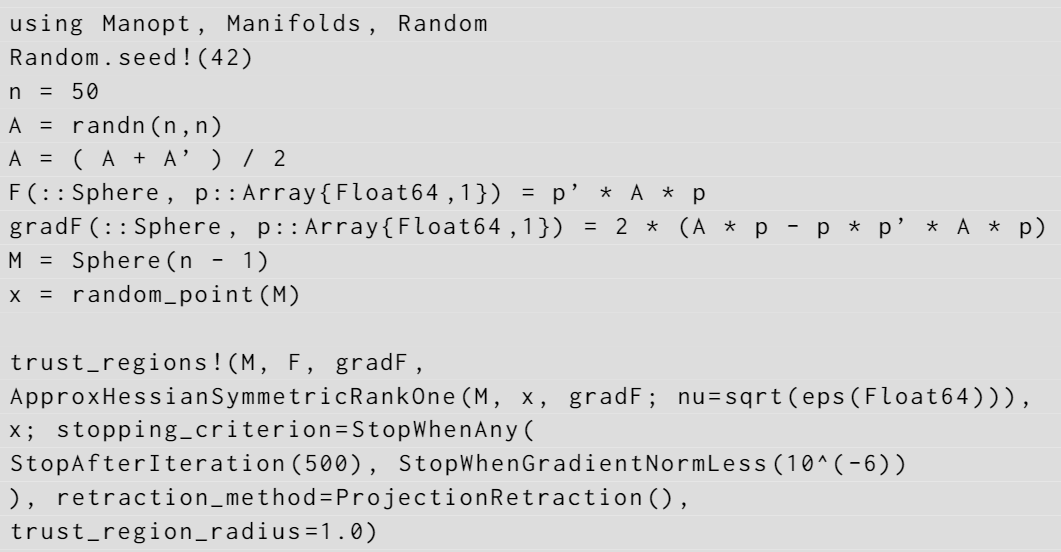
\includegraphics[width=11cm]{img/Rayleigh_Experiment_2.png}
    \end{center}
\end{frame}

\begin{frame}{Results}
    Comparison of ... in an average of 10 random runs:
    \begin{table}[H]
        \resizebox{\textwidth}{!}{
            \begin{tabular}{lcccccc}
                \toprule
                Manifold & \multicolumn{2}{c}{$\mathbb{S}^{49}$}& \multicolumn{2}{c}{$\mathbb{S}^{99}$} & \multicolumn{2}{c}{$\mathbb{S}^{199}$}\\ 
                \cmidrule(lr){2-3} \cmidrule(lr){4-5} \cmidrule(lr){6-7}
                Quadratic term & Newton & SR1 & Newton & SR1 & Newton & SR1 \\ 

                Time in ms & $4.5$ & $17.0$ & $54.2$ & $80.2$ & $245.5$ & $269.4$\\ 
                Iterations & $9.2$ & $41.5$ & $10.2$ & $70.1$ & $10.5$ & $83.1$ \\
                \bottomrule
            \end{tabular}
        }
    \end{table}
\end{frame}

\section{Conclusion}

\begin{frame}{Conclusion}
    \begin{itemize}
        \item RTR-SR1 method is generalized to Riemannian manifolds.
        \item SR1 approximation is implemented in Manopt.jl.
        \item Next step: Implementing limited-memory variant.
    \end{itemize}
    \vspace{10mm}
    \begin{center}
        Thank you for your attention! 
    \end{center}
\end{frame}

\end{document}
